\documentclass[11pt]{article}
\usepackage[margin=1.05in]{geometry}
\usepackage{amsmath,amssymb,amsthm}
\usepackage{booktabs}
\usepackage{graphicx}
\usepackage[colorlinks=true,linkcolor=blue,citecolor=blue,urlcolor=blue]{hyperref}

\newcommand{\voles}{\texttt{voles}}
\newcommand{\dd}{\,\mathrm{d}}
\newcommand{\kw}[1]{\texttt{#1}}
\newtheorem{theorem}{Theorem}
\newtheorem{corollary}{Corollary}
\newtheorem{lemma}{Lemma}

\title{Deterministic Gauss--Jacobi quadrature\\ for weakly singular weight
blocks}
\author{Notes accompanying branch \texttt{gauss-jacobi-singular-quadrature}}
\date{August 2026}

\begin{document}
\maketitle

\begin{abstract}
\noindent
The callable-input \voles{} solvers assemble their weight tensors by
integrating the kernel against local polynomial basis functions on each mesh
interval. Blocks touched by a declared kernel singularity have until now
required adaptive (QUADPACK) quadrature, whose results are reproducible only
to its tolerance; under the strict floating-point policy those blocks were
therefore re-evaluated per mesh row, leaving an $O(M)$
adaptive-quadrature cost that dominates weakly singular builds, or --- with
the opt-in \kw{reuse\_adaptive\_blocks} flag --- reused at the price of
tolerance-level deviations. This note documents the replacement: when the
user declares the singularity's power-law exponent
($K(u)\sim|u-u_0|^{-\alpha}$) via
\kw{kernel\_singularity=\{location:\ alpha\}}, singular blocks are evaluated
by \emph{fixed-order Gauss--Jacobi rules} whose weight function absorbs the
singular factor exactly. The rule is deterministic, so the blocks join the
Toeplitz fast path's reuse set and Abel-kernel assembly becomes as fast as
smooth-kernel assembly --- with no flag and no tolerance-level reuse. The
same two-order acceptance check that guards the smooth Gauss--Legendre path
guards the new rule, so a mis-declared exponent degrades \emph{bitwise} to
the previous adaptive behavior. A 56-case A/B battery against the pre-change
build confirms: all 46 legacy-form cases are bit-identical, scalar
deviations for the new form are bounded by the check tolerance
(worst $1.2\times10^{-9}$ scale-relative), and the vector path becomes
\emph{more} accurate --- its deviation ($1.3\times10^{-8}$) is shown by an
independent diagonalization experiment to be entirely the old
\kw{quad\_vec} path's error.
\end{abstract}

\section{Interface}

All three callable-input solvers accept exponents through the existing
keyword:
\begin{center}
\kw{function\_solve\_*(\dots, kernel\_singularity=\{0.0:\ 0.5\})}
\end{center}
Accepted forms, in increasing generality: \kw{None}; a bare float location
(u-coordinate, $u=t-s$); a list of locations; a dict
\kw{\{location:\ alpha\}}; a list mixing bare locations and
\kw{(location, alpha)} pairs; a callable \kw{t -> [s-locations]}. Bare
locations (and callables) keep the historical adaptive behavior, bit for
bit. Exponents must satisfy $0<\alpha<1$ (integrable power-law
singularities); pairs must be nested --- a flat tuple \kw{(0.0, 0.5)} is,
as before, two bare locations.

A companion keyword \kw{singular\_quadrature='auto'|'adaptive'} (default
\kw{'auto'}) selects the policy: \kw{'auto'} uses Gauss--Jacobi on blocks
whose declared singularities all carry exponents; \kw{'adaptive'} forces
the historical adaptive path even when exponents are declared (an escape
hatch and an A/B lever --- enforced by test to be bit-identical to the
bare-location call).

Guarantees, enforced by tests: every historical call form is bit-identical
to the pre-change build; smooth kernels are untouched; a wrong declared
exponent falls back, again bit-identically, to the adaptive path
(Section~\ref{sec:check}).

\section{The problem: singular weight blocks}

Write the mesh $0=t_0<t_1<\dots<t_M=T$, collocation nodes
$\tau_{n,i}=t_n+c_i h_n$, and local basis polynomials $L_k$ on the
normalized interval. Every entry of the weight tensor is a block integral
\begin{equation}
  W[n,i,l,k] \;=\; \int_{t_l}^{b}\! K(\tau_{n,i}-s)\,
  L_k\!\Bigl(\tfrac{s-t_l}{h_l}\Bigr)\dd s,
  \qquad b = \min(t_{l+1},\,\tau_{n,i}).
  \label{eq:block}
\end{equation}
For a weakly singular kernel, $K(u) = |u-u_0|^{-\alpha}\,\varphi(u)$ with
$\varphi$ smooth near the declared point $u_0$ (the Abel case is $u_0=0$,
$\alpha=\tfrac12$, $\varphi$ smooth). The singular $s$-location seen from
collocation point $\tau$ is $s^\ast = \tau-u_0$. Blocks containing
$s^\ast$ (in the interior or at an endpoint) cannot be handled by the
smooth path's Gauss--Legendre rules --- the integrand is unbounded --- and
have historically gone to per-basis QUADPACK, with two costs: each call is
$\sim$two orders of magnitude more expensive than a fixed-order rule, and
the result is reproducible only to the requested tolerance, which excludes
these blocks from the Toeplitz fast path's reuse set under the strict
floating-point policy.

The observation driving this branch: \emph{the singular factor is known
exactly once $\alpha$ is declared}. A quadrature rule built for the weight
$|s-s^\ast|^{-\alpha}$ integrates it analytically; only the smooth
remainder $\varphi\cdot L_k$ is approximated. This is the classical
product-integration idea, realized with Gauss--Jacobi nodes.

\section{The algorithm}

\subsection{Gauss--Jacobi rules}
For exponents $a,b>-1$ the Jacobi weight on $[-1,1]$ is
$w^{(a,b)}(x)=(1-x)^a(1+x)^b$. The $n$-point Gauss--Jacobi rule has nodes
$x_q$ at the roots of the degree-$n$ Jacobi polynomial $P_n^{(a,b)}$
(orthogonal with respect to $w^{(a,b)}$) and weights $w_q>0$ such that
\begin{equation}
  \sum_{q=1}^{n} w_q\, g(x_q) \;=\; \int_{-1}^{1} w^{(a,b)}(x)\, g(x)\dd x
  \qquad\text{exactly for all polynomials } g,\ \deg g \le 2n-1.
  \label{eq:gj}
\end{equation}

\begin{theorem}[Gaussian exactness]\label{thm:exact}
Property \eqref{eq:gj} holds for any weight $w\ge0$ with finite moments,
with nodes at the roots of the degree-$n$ orthogonal polynomial $\pi_n$
and weights $w_q = \int w\,\ell_q$ for the Lagrange cardinal polynomials
$\ell_q$ of the node set.
\end{theorem}
\begin{proof}
Divide $g = q\,\pi_n + r$ with $\deg q,\deg r\le n-1$. Orthogonality gives
$\int w\,q\,\pi_n = 0$, and $\pi_n(x_q)=0$ kills the same term in the sum,
so both sides equal the degree-$(n-1)$ statement for $r$; that in turn
holds because $r=\sum_q r(x_q)\ell_q$ exactly and $w_q=\int w\,\ell_q$ by
definition. Positivity of $w_q$ follows from applying the rule to
$\ell_q^2$ (degree $2n-2\le 2n-1$).
\end{proof}

We obtain nodes and weights from \kw{scipy.special.roots\_jacobi(n, a, b)},
computed by the Golub--Welsch eigenvalue method --- deterministic for fixed
$(n,a,b)$, cached per triple.

\subsection{Folded weights: singular blocks in smooth-block form}
\label{sec:folded}
Consider a block $[A,B]$ whose integrand carries singular factors
$(B-s)^{-\alpha_R}$ and/or $(s-A)^{-\alpha_L}$ at its endpoints (either
exponent may be $0$). Map $s = \tfrac{A+B}{2} + \eta x$ with
$\eta=\tfrac{B-A}{2}$, so $B-s=\eta(1-x)$ and $s-A=\eta(1+x)$. For the
full integrand $F(s)=K(\tau-s)L(s)$ with
$K = |s-s^\ast|^{-\alpha}\varphi$,
\begin{equation}
  \int_A^B F \dd s
  \;=\; \eta \int_{-1}^{1} (1-x)^{-\alpha_R}(1+x)^{-\alpha_L}
  \underbrace{\bigl[(1-x)^{\alpha_R}(1+x)^{\alpha_L}
  F\bigl(s(x)\bigr)\bigr]}_{=:G(x),\ \text{smooth}}\dd x
  \;\approx\; \eta \sum_q \widetilde w_q\, F\bigl(s(x_q)\bigr),
  \label{eq:folded}
\end{equation}
where the \emph{folded weights}
$\widetilde w_q = w_q (1-x_q)^{\alpha_R}(1+x_q)^{\alpha_L}$ use the
Gauss--Jacobi weights for $w^{(-\alpha_R,-\alpha_L)}$. The middle equality
is an identity; the approximation applies rule \eqref{eq:gj} to $G$.
$G$ is smooth because the folded factors cancel the singular factor of $K$
analytically: near $x=1$,
$K \sim (\eta(1-x))^{-\alpha_R}\varphi$, so
$G \sim \eta^{-\alpha_R}\varphi\,L$.

The practical consequence of \eqref{eq:folded} is that a singular block is
accumulated \emph{exactly like a smooth Gauss--Legendre block} --- raw
kernel values at the nodes, dotted with cached weights, times $\eta$ ---
with $\widetilde w$ in place of the GL weights. One kernel sweep per
order serves every basis function of the block simultaneously, as on the
smooth path. For $\alpha_R=\alpha_L=0$ the folding is a no-op and the rule
\emph{is} Gauss--Legendre.

\begin{corollary}[Exactness for pure power kernels]\label{cor:pure}
If $K(u)=|u-u_0|^{-\alpha}$ exactly (i.e.\ $\varphi\equiv1$) and $L$ is a
polynomial of degree $\le 2n-1$, the $n$-point folded rule evaluates the
block integral \eqref{eq:block} exactly (up to rounding).
\end{corollary}
\begin{proof}
$G(x) = \eta^{-\alpha}L(s(x))$ is then itself a polynomial of degree
$\deg L$, and Theorem~\ref{thm:exact} applies.
\end{proof}

For $K = |u-u_0|^{-\alpha}\varphi(u)$ with $\varphi$ analytic in a
neighborhood of the block, $G$ is analytic and the rule converges
geometrically in $n$: the error after $n$ points is
$O(\rho^{-2n})$ with $\rho>1$ the Bernstein-ellipse parameter of
$\varphi\cdot L$ --- the same regime that makes the smooth path's GL orders
6/8 far more accurate than the $10^{-9}$ acceptance threshold in practice.

\subsection{Block splitting}
Each singular block is split at its interior declared points; each piece
then has singularities only at endpoints, handled by \eqref{eq:folded}:
\begin{itemize}
  \item \textbf{Diagonal blocks} ($u_0=0$): $s^\ast=\tau=B$; one piece,
  $\alpha_R=\alpha$, $\alpha_L=0$.
  \item \textbf{Interior} $s^\ast\in(A,B)$: two pieces $[A,s^\ast]$,
  $[s^\ast,B]$ with the exponent on the shared endpoint --- the two
  one-sided halves of $|s-s^\ast|^{-\alpha}$.
  \item \textbf{Both endpoints singular} (two declared points landing on
  the two ends): a single piece with both exponents --- the general Jacobi
  weight handles it natively.
\end{itemize}
Degenerate declarations (two singular points within the classification
tolerance of each other) are not eligible and take the adaptive path
unchanged.

\subsection{Endpoint-anchored kernel arguments}
The kernel is evaluated at $u_q=\tau-s_q$. Computed naively, this
subtraction cancels catastrophically near a singular endpoint (the node
closest to a diagonal singularity has
$u\sim\eta(1-x_{\max})\ll\tau$). The implementation instead uses the
identity
\[
  \tau - s_q \;=\; (\tau - B) + \eta\,(1 - x_q),
\]
in which $\tau-B$ is computed once per piece and is \emph{exactly zero}
for diagonal blocks ($B=\tau$ bitwise), so the argument is formed from
$\eta(1-x_q)$ at full relative precision. For pieces ending at an interior
singular point, $\tau-B$ is the declared $u_0$ up to one rounding.

\subsection{The acceptance check and fallback}\label{sec:check}
The smooth path accepts a Gauss--Legendre block only if its order-6 and
order-8 estimates agree to $10^{-9}$ (relative, floored at 1), falling
back per basis function to QUADPACK otherwise. The Gauss--Jacobi path
inherits the same check verbatim: the block is evaluated at orders 6 and
8, the order-8 value is stored, and any basis function failing
$|v_6-v_8|\le 10^{-9}\max(1,|v_8|)$ is recomputed by \emph{exactly the
adaptive call the pure-adaptive path would make} --- same integrand
closure, same \kw{quad} options, same interior \kw{points} list. Hence:
\begin{itemize}
  \item A correctly declared exponent on a kernel with smooth $\varphi$:
  both orders agree to near machine precision; the block is accepted and
  is deterministic.
  \item A wrong exponent (e.g.\ $\alpha=0.25$ declared on $u^{-1/2}$):
  $G$ retains a $u^{-1/4}$ singularity, the orders disagree, and every
  singular block falls back --- the solve is then \emph{bit-identical} to
  the bare-location call (verified by test and by the A/B battery).
  \item A non-power-law or composite singularity (e.g.\
  $K=|u-u_0|^{-1/2}+1$, whose regularized remainder is not smooth): same
  graceful fallback, per block and per basis function.
\end{itemize}
The check is the safety net that lets \kw{'auto'} be the default: the
worst case of a bad declaration is the historical behavior at the
historical cost.

\section{Interaction with the Toeplitz fast path}

On a uniform mesh with a convolution kernel the weight tensor is Toeplitz
in $(n,l)$ and is assembled from one integrated row; only blocks whose
values are \emph{deterministic} (fixed-order rule, check passed) may be
copied across rows under the strict policy, because a copy must reproduce
a per-row evaluation to rounding. Adaptive blocks failed that criterion
and were re-run per row --- the $O(M)$ cost that motivated the
\kw{reuse\_adaptive\_blocks} flag. Gauss--Jacobi blocks \emph{are}
deterministic: they join the reuse set exactly as GL-clean blocks do, the
per-row recomputation loop finds nothing left to do, and the singular
build inherits the smooth build's cost structure --- one integrated row,
one band-diagonal copy. Equal-lag singular blocks are now bitwise equal by
construction, eliminating even the $\sim3\times10^{-10}$ equal-block
scatter that QUADPACK's branch-dependent adaptivity produced (see the
\kw{adaptive\_reuse\_notes} for that measurement). Off the fast path
(graded or otherwise non-uniform meshes) the rules still apply per block
--- deterministic and cheap, just without cross-row reuse.

With exponents declared, \kw{reuse\_adaptive\_blocks} has essentially
nothing left to act on; the flag remains for bare-location declarations.

\section{Verification}

Three layers, following the branch's standing playbook.

\paragraph{Rule exactness.} Unit tests verify the folded rule against
closed-form Beta-function integrals,
$\int_A^B (B-s)^{-\alpha}(s-A)^k \dd s
= (B-A)^{k+1-\alpha}B(k{+}1,1{-}\alpha)$ (and the two-sided analogue), to
$10^{-13}$ relative for polynomial degrees through 11 at order 6 and
$\alpha\in\{0.25,0.5,0.9\}$; and that the $(0,0)$ rule reproduces
Gauss--Legendre to $10^{-14}$.

\paragraph{Weight tensors.} For $K=u^{-1/2}(2+\cos u)$ (smooth factor
times the declared power) the full Gauss--Jacobi weight tensor matches an
\kw{epsabs=epsrel=}$10^{-12}$ adaptive reference to $10^{-10}$
scale-relative; likewise for the pure two-sided interior kernel
$|u-0.5|^{-1/2}(2+\cos u)$. The vector builder reproduces the scalar
weights entrywise ($10^{-13}$) for a constant-matrix-times-scalar kernel,
which certifies the vector path without inheriting \kw{quad\_vec} errors.

\paragraph{A/B battery.} Both builds (baseline \texttt{5960786} in a git
worktree vs.\ the branch) ran an identical 56-case battery: every
test-suite problem spec through its solver at $M=20$ and $M=80$, plus
graded-mesh, list/tuple/callable-form, reuse-flag, vector, complex, and
continuous-method cases.
\begin{itemize}
  \item \textbf{Legacy forms (46 cases): all bit-identical}
  (\kw{np.array\_equal}). The refactor is a strict no-op for every
  historical call.
  \item \textbf{Dict forms (10 cases):} the baseline's normalization
  iterates a dict and sees bare keys, so the same invocation ran adaptive
  on the baseline and Gauss--Jacobi on the branch --- a direct
  measurement of the policy deviation. Scalar cases: worst
  $1.2\times10^{-9}$ scale-relative (the VIE-1 continuous case; typical
  $10^{-11}$), bounded by the acceptance tolerance as designed.
  \item \textbf{Vector attribution:} the coupled $2\times2$ Abel case
  (negative-definite coupling --- positive eigenvalues would inflate the
  solution Mittag-Leffler-fast and make absolute comparisons meaningless)
  deviated by $1.3\times10^{-8}$. Diagonalizing the system
  ($C=V\Lambda V^{-1}$) reduces it to scalar solves --- independently
  verified to $10^{-10}$ --- whose recombination is an external
  reference: the \emph{old} path sits $1.3\times10^{-8}$ from it, the new
  path $2.8\times10^{-15}$. The deviation is entirely the old
  \kw{quad\_vec} tolerance error; the new path removes it.
\end{itemize}

\section{Benchmarks}

Abel VIE-2 ($K=u^{-1/2}$, $y=\sqrt t$, $T=1$, $p=3$), uniform meshes,
nodal output, best-of-3 timings after warm-up, Apple-silicon laptop:

\begin{center}
\begin{tabular}{lrrrrrr}
\toprule
$M$ & 40 & 80 & 160 & 320 & 640 & 1280\\
\midrule
adaptive (strict, per-row)      & 0.115 & 0.230 & 0.458 & 0.919 & 1.878 & 3.781\\
Gauss--Jacobi (strict)          & 0.006 & 0.012 & 0.024 & 0.051 & 0.107 & 0.237\\
\kw{reuse\_adaptive\_blocks}    & 0.007 & 0.009 & 0.012 & 0.020 & 0.044 & 0.097\\
smooth kernel (reference)       & 0.001 & 0.002 & 0.005 & 0.012 & 0.030 & 0.080\\
\midrule
speedup, GJ vs adaptive         & $19\times$ & $19\times$ & $19\times$
                                & $18\times$ & $18\times$ & $16\times$\\
\bottomrule
\end{tabular}
\end{center}

\noindent
The residual factor of $\sim$3 between the Gauss--Jacobi and smooth builds
is not the singular blocks (those now cost the same as smooth ones): it is
the \emph{near}-singular lag-1 blocks at interior collocation nodes, where
the singularity sits just outside the block, the GL two-order check fails,
and the per-basis adaptive fallback runs per row as it always has. That is
also why \kw{reuse\_adaptive\_blocks} remains $\sim$2$\times$ faster at
large $M$: it reuses those fallback blocks at tolerance level, outside the
strict policy. Closing the gap deterministically (e.g.\ composite or
higher-order rules for near-singular blocks, under the same check) is
possible future work.

The Gauss--Jacobi build tracks the smooth-kernel build within a small
factor across the sweep --- the ``singular assembly at smooth-assembly
cost'' target --- while the strict adaptive path pays its $O(M)$
per-row adaptive cost and the reuse flag pays adaptive cost once.
Figure~\ref{fig:speedup} shows the sweep; Figure~\ref{fig:diffs} the
A/B deviations.

\begin{figure}[htbp]
  \centering
  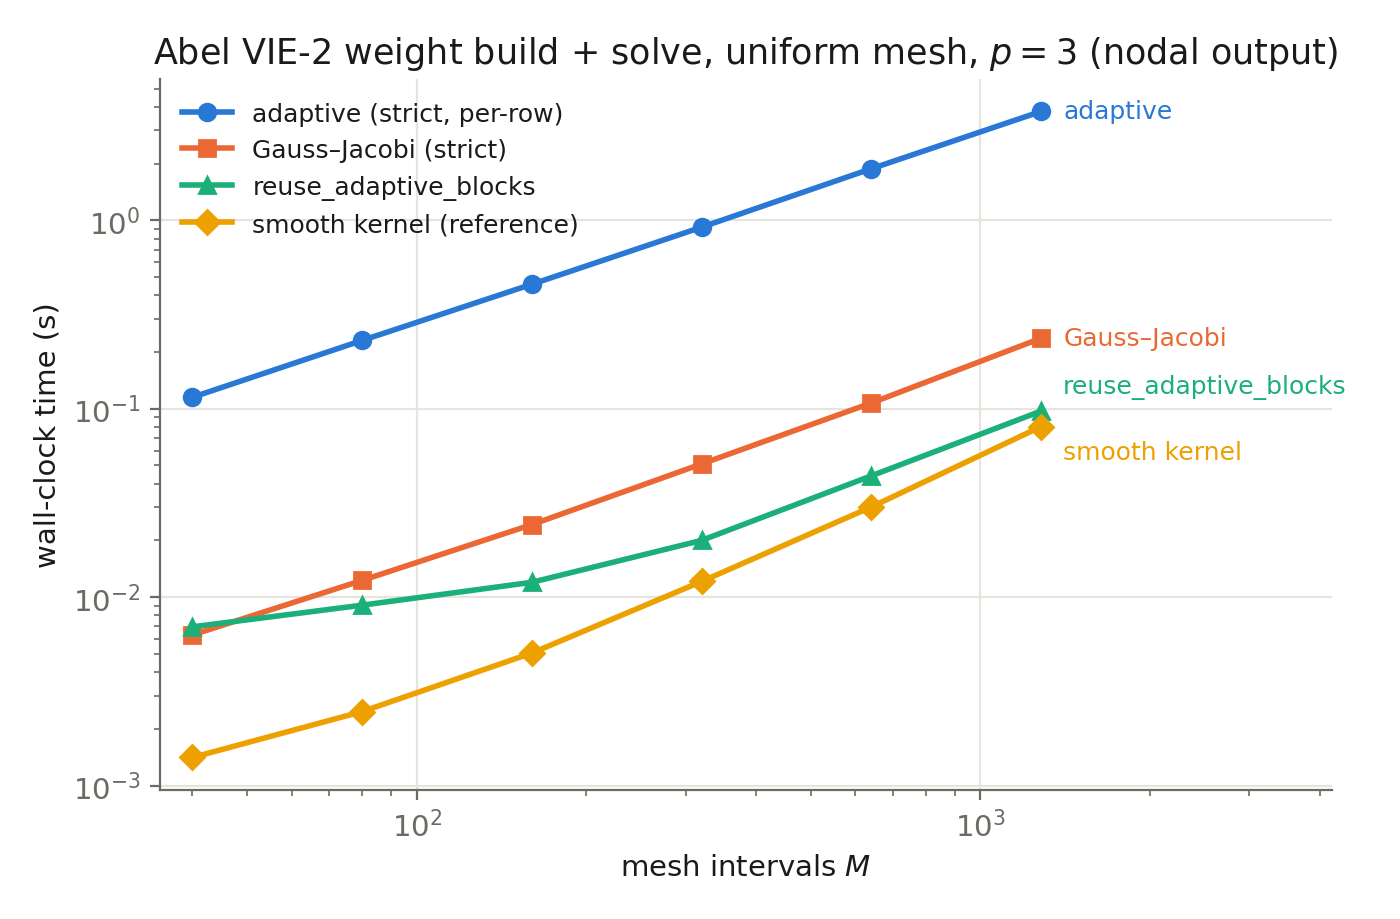
\includegraphics[width=0.85\textwidth]{plot_gj_speedup.png}
  \caption{Wall-clock time vs.\ mesh size for the four configurations.}
  \label{fig:speedup}
\end{figure}

\begin{figure}[htbp]
  \centering
  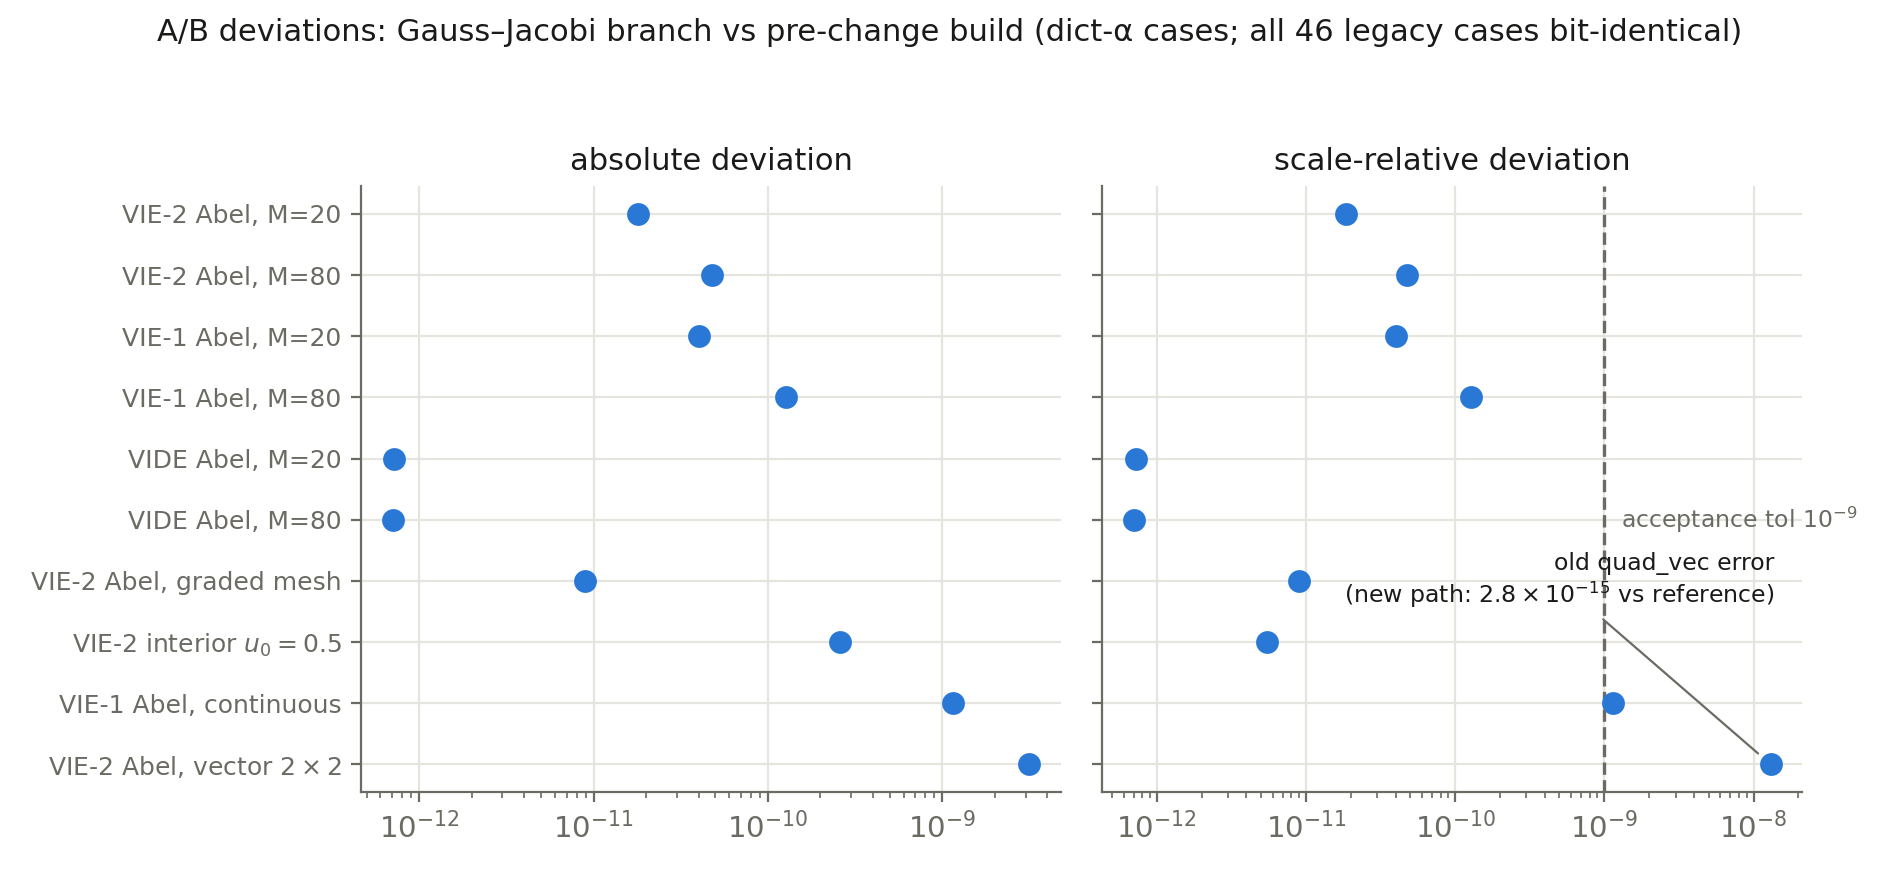
\includegraphics[width=0.95\textwidth]{plot_gj_differences.png}
  \caption{A/B deviations, new vs.\ pre-change build: absolute (left) and
  scale-relative (right). Legacy-form cases are identically zero and
  omitted; the dashed line is the $10^{-9}$ acceptance tolerance. The
  vector case's excess is the old path's \kw{quad\_vec} error
  (Section~5).}
  \label{fig:diffs}
\end{figure}

\section{Floating-point and accuracy caveats}

Kept to the end deliberately: none of the following affects the algorithm
above, only how its output relates to the previous code's output.

\begin{itemize}
  \item \textbf{Nature of the deviation.} Gauss--Jacobi and QUADPACK both
  approximate the same exact integral; neither is the other's truth.
  Declaring an exponent changes singular-block values within the
  acceptance envelope ($10^{-9}$ relative, floored at 1) --- the same
  epistemic status the smooth path's GL-accepted blocks have always had
  relative to hypothetical adaptive values. For pure power kernels the
  new values are \emph{exact} up to rounding
  (Corollary~\ref{cor:pure}); for smooth $\varphi$ they are typically
  $10^{-12}$ or better, i.e.\ closer to the true integral than the
  default-tolerance adaptive values they replace.
  \item \textbf{Vector path.} The old vector singular blocks used
  \kw{quad\_vec}, whose errors ($\sim10^{-8}$ scale-relative in the A/B
  battery) dominate any comparison. Deviations there are an accuracy
  \emph{improvement}, demonstrated by the diagonalization experiment.
  \item \textbf{Determinism and reuse.} Equal-lag singular blocks are now
  bitwise equal (one evaluation, band-copied). Per-row re-evaluation on
  the old path produced values scattered by up to $3.4\times10^{-10}$
  between equal blocks; that scatter is gone, not merely reduced.
  \item \textbf{No silent activation.} Every path to the new rule runs
  through an argument form the old code treated as bare locations or
  rejected; plain floats, lists, and callables are bit-identical to the
  pre-change build (46/46 A/B cases), as is
  \kw{singular\_quadrature='adaptive'}.
  \item \textbf{When not to declare $\alpha$.} If the exponent is unknown,
  uncertain, or the singularity is not a power law (logarithmic, say),
  declare the bare location: the adaptive path remains first-class. A
  wrong declaration costs nothing but the failed check --- the fallback
  is bitwise the adaptive result --- but a \emph{nearly} right exponent
  on a marginally smooth remainder could in principle pass the check at
  $10^{-9}$ while being less accurate than adaptive at its own
  tolerance; the check tolerance is the guarantee, not the typical error.
\end{itemize}

\paragraph{Looking ahead.} These rules are the quadrature substrate for
the planned uniform-mesh singular-basis augmentation (the successor to
the graded-mesh roadmap item): the moment integrals
$\int K(\tau-s)\,s^{\gamma}\dd s$ of the augmentation's nonpolynomial
basis functions carry the same endpoint singularities and will be
computed by the same folded-weight machinery.

\end{document}
